\documentclass[specialist,
               substylefile = spbu_report.rtx,
               subf,href,colorlinks=true, 12pt]{disser}

\usepackage[a4paper,
            mag=1000, includefoot,
            left=3cm, right=1.5cm, top=2cm, bottom=2cm, headsep=1cm, footskip=1cm]{geometry}
\usepackage[T2A]{fontenc}
\usepackage[utf8]{inputenc}
\usepackage[english,russian]{babel}
\ifpdf\usepackage{epstopdf}\fi

% Точка с запятой в качестве разделителя между номерами цитирований
%\setcitestyle{semicolon}


% Включать подсекции в оглавление
\setcounter{tocdepth}{2}

\graphicspath{{fig/}}

%----------------------------------------------------------------
\begin{document}

%
% Титульный лист на русском языке
%

% Название организации
\institution{%
    Санкт-Петербургский государственный университет \\
    Прикладная математика и информатика \\
    Прикладная кибернетика
}

\title{Научная иследовательская разбота}

% Тема
\topic{\normalfont\scshape%
Cравние на синтетических данных и на данных с Kaggle методов для рассчёта доверительных интервалов для 90, 99 квантилей}

% Автор
\author{Кривоносов Тимофей Игоревич}

% Научный руководитель
\sa       {М.\,В.~Юлдашев}
\sastatus {д.\,ф.-м.\,н., профессор}

% Рецензент
\rev      {П.\,П.~Петров}
\revstatus{к.\,ф.-м.\,н., доцент}

% Город и год
\city{Санкт-Петербург}
\date{\number\year}

\maketitle

\newpage
\tableofcontents
\newpage
\section{Введение}
В современном мире статистический анализ играет важную роль во многих областях, от науки до бизнеса. При работе с данными мы часто сталкиваемся с необходимостью оценки параметров и построения доверительных интервалов для различных квантилей распределений. Квантили представляют собой значения, разделяющие вероятностное распределение на равные части.

В данной курсовой работе мы сосредоточимся на сравнении методов для расчета доверительных интервалов для 90-го и 99-го квантилей на основе синтетических данных и данных, предоставленных платформой Kaggle. Синтетические данные являются созданными искусственным образом наборами данных, которые позволяют нам контролировать различные аспекты, такие как распределение, объем выборки и т.д. Данные, полученные с Kaggle, представляют собой реальные данные, предоставленные сообществом пользователей этой платформы.

Для синтезирования данных и проверки методов поиска доверительных интервалов для 90 и 99 квантилей в задаче сравнения производительности и задержки (latency), проведу следующие шаги:

\begin{itemize}
 
\item  Собрать данные: Запустите эксперименты или тесты, которые измеряют производительность и задержку вашей системы. Запишите результаты для каждого теста.

\item Подготовить выборки: Создайте выборки из результатов тестов, соответствующие каждому методу или условию, которое вы хотите сравнить. Например, если вы сравниваете два разных алгоритма, создайте две выборки, содержащие результаты для каждого алгоритма.

\item Анализировать выборки: Используйте статистические методы для анализа выборок и вычисления доверительных интервалов. Для нахождения доверительного интервала 90\% квантили, найдите 5-й и 95-й перцентили выборки. Для доверительного интервала 99\% квантили найдите 0.5-й и 99.5-й перцентили выборки.

\item  Проверьте методы поиска доверительных интервалов: Сравните результаты, полученные различными методами поиска доверительных интервалов. Убедитесь, что методы возвращают адекватные и интерпретируемые результаты.

\item Интерпретация результатов: Проанализируйте полученные доверительные интервалы и сделайте выводы относительно производительности и задержки системы. Например, если интервалы значительно отличаются для двух методов, это может указывать на значимые различия между ними.
\end{itemize}

Основной целью нашего исследования является провести сравнительный анализ методов расчета доверительных интервалов для выбранных квантилей на основе обоих типов данных. Это позволит нам оценить, насколько точно и надежно эти методы работают в различных условиях и с разными типами данных.

Ожидается, что результаты данного исследования помогут нам лучше понять применимость и эффективность различных методов для расчета доверительных интервалов на основе разных типов данных, что может быть полезным при принятии статистических решений в реальных ситуациях.
\newpage
\section{Методы нахождения доверительных интервалов}
Доверительные интервалы являются важным инструментом в статистике и анализе данных. Они предоставляют информацию о диапазоне значений, в пределах которого с определенной вероятностью находится истинное значение параметра популяции. Методы нахождения доверительных интервалов разрабатываются для различных статистических оценок, таких как среднее, медиана, квантили и дисперсия.

В данном контексте существует несколько методов, включая аналитические, бутстреп и другие. Аналитические методы обычно требуют явных аналитических моделей и предположений о распределении данных. Бутстреп - это метод ресемплинга, который позволяет оценивать доверительные интервалы на основе эмпирических данных без явных предположений.

В этом контексте, мы будем исследовать различные методы нахождения доверительных интервалов и сравнивать их производительность в оценке статистических параметров в задачах анализа производительности и задержки.

\subsection{Наивный подход}

Наивный подход (или иногда "классический подход") при поиске доверительного интервала предполагает использование простых формул или методов для оценки параметров популяции или статистических характеристик на основе имеющихся данных без учета сложных статистических моделей или методов ресемплинга.

Основные черты наивного подхода:
\begin{itemize}
    \item Простота: Наивный подход обычно предполагает использование простых статистических оценок, таких как выборочное среднее, выборочная дисперсия, медиана и квантили, без необходимости в более сложных методах.
    \item Явные формулы: В большинстве случаев наивные методы имеют явные аналитические формулы для вычисления оценок и доверительных интервалов. Например, доверительный интервал для среднего значения в выборке с известной дисперсией может быть вычислен с использованием формулы Z-критерия.
    \item Предположения о распределении: Наивные методы часто основываются на предположениях о распределении данных, таких как нормальное распределение. Они могут быть неустойчивыми к нарушениям этих предположений.
    \item Ограниченная гибкость: Наивные методы могут быть ограничены в способности учитывать сложные зависимости в данных или рассматривать данные, не подчиняющиеся стандартным распределениям.
\end{itemize}

Наивный подход полезен, когда у вас есть хорошие основания для использования простых методов, и когда они дают приемлемые результаты. Однако в случае сложных данных или данных, не соответствующих предполагаемым распределениям, наивный подход может быть недостаточным и неустойчивым. В таких случаях более сложные методы, такие как бутстреп или аналитические модели, могут быть более надежными.

Алгоритм нахождения доверительного интервала с его помощью обычно включает следующие шаги:
\begin{itemize}
    \item Шаг 1: Собрать выборку данных. Это могут быть измерения, результаты эксперимента или другие данные, на основе которых вы хотите построить доверительный интервал.
    \item Шаг 2: Выбрать уровень доверия (например, 95 \% или 99\%). Уровень доверия определяет, с какой вероятностью истинное значение параметра популяции находится внутри доверительного интервала.
    \item Шаг 3: Определить статистическую оценку параметра. Наивный подход часто использует выборочные статистики, такие как выборочное среднее $\bar{x}$ или выборочная медиана, для оценки параметра популяции.
    \item Шаг 4: Определить стандартную ошибку. Стандартная ошибка (SE) измеряет разброс выборочной статистики и зависит от объема выборки. Для среднего значения это может быть вычислено как стандартное отклонение выборки, деленное на корень из размера выборки ($SE = \sigma / \sqrt{n} $, где $\sigma$ - стандартное отклонение популяции).
    \item Шаг 5: Определить критическое значение. Критическое значение определяет, какие значения статистики считаются "достаточно экстремальными" для данного уровня доверия. Наивный подход обычно использует критические значения из стандартных распределений, таких как Z-распределение или t-распределение.
    \item Шаг 6: Вычислить доверительный интервал. Доверительный интервал определяется как оценка параметра плюс/минус критическое значение, умноженное на стандартную ошибку. Для среднего значения (наивный метод):
    
    Доверительный интервал = оценка параметра ± (критическое значение * SE)

\end{itemize}

Пример:

Предположим, у нас есть выборка из 30 измерений длины стержня, и мы хотим построить 95 \% доверительный интервал для средней длины стержня. Стандартное отклонение выборки равно 2 см.

\begin{itemize}
    \item Выборка данных: [10, 11, 12, 14, 15, 11, 13, 12, 14, 15, 15, 13, 12, 13, 14, 16, 17, 18, 15, 12, 13, 12, 14, 15, 16, 17, 16, 13, 12, 14]
    \item Уровень доверия: 95\%
    \item Статистическая оценка: Выборочное среднее $bar{x}$ = 14
    \item Стандартная ошибка: $SE = 2 / \sqrt{30} \approx 0.365$
    \item Критическое значение: Для 95\% доверия с использованием Z-распределения, критическое значение равно примерно 1.96.
    \item Вычисление доверительного интервала: 
    
    Доверительный интервал = 14 ± (1.96 * 0.365)$ \approx $ [13.29, 14.71]
    \end{itemize}
    Таким образом, с 95\% уровнем доверия мы можем утверждать, что средняя длина стержня находится в интервале от 13.29 см до 14.71 см.

\subsection{Бустерэп}
Бутстрэп - это метод статистической ресемплинга, который используется для оценки дисперсии и доверительных интервалов для статистических оценок, когда точное аналитическое решение сложно или невозможно. Он широко применяется в статистике и машинном обучении для решения различных задач, таких как оценка параметров, построение доверительных интервалов и проверка гипотез. Вот как он работает:
\begin{itemize}
    \item Создание репликаций: Из вашей исходной выборки размером N (обычно с заменой) генерируются множество новых выборок (репликаций). Количество репликаций, обычно обозначаемое как B, может быть выбрано пользователем и обычно составляет несколько сотен или тысяч.
    \item Оценка интересующей статистики: Для каждой из B репликаций, вы оцениваете интересующую вас статистику. Это может быть, например, среднее, медиана, доля, стандартное отклонение, коэффициент корреляции или что-либо еще в зависимости от вашей задачи.
    \item Анализ распределения: После оценки статистики для каждой репликации, вы получаете распределение значений этой статистики на основе бутстреп-выборок.
    \item Построение доверительных интервалов: Из анализа этого распределения можно построить доверительные интервалы для вашей статистики. Наиболее распространенным методом для этого является метод "перцентильного доверительного интервала", который использует квантили распределения.
\end{itemize}
Пример использования метода:
\newline
Предположим, у нас есть выборка размером 100 наблюдений и мы хотим построить доверительный интервал для среднего значения. Мы можем применить метод бутстрэп следующим образом:

\begin{itemize}
    \item Создаем множество бутстрэп-выборок путем случайного выбора 100 наблюдений из исходной выборки с возвращением.
    \item Для каждой бутстрэп-выборки вычисляем среднее значение.
    \item Полученные средние значения образуют распределение, которое отражает неопределенность вокруг истинного среднего значения.
    \item Используем полученное распределение для построения доверительного интервала, например, 95\% доверительного интервала будет содержать средние значения, лежащие между 2.5-м и 97.5-м процентилями этого распределения.
\end{itemize}

Таким образом, метод бутстрэп позволяет оценить статистическую неопределенность и построить доверительные интервалы для различных параметров на основе анализа повторных выборок из исходной выборки.

\subsection{Дельта подход}

Дельта-метод - это статистический метод, используемый для оценки дисперсии и построения доверительных интервалов для функций случайных величин на основе их оценок и производных. Основное предположение метода Дельта состоит в том, что оценки параметров близки к нормальному распределению.


Доказательство метода Дельта является более сложным и требует математической формализации и использования разложения в ряд Тейлора. Давайте представим общий контур доказательства метода Дельта, который включает следующие шаги:

Предположим, у нас есть функция случайной величины X, которую мы обозначим как g(X), и мы хотим оценить ожидание этой функции, то есть E[g(X)].

\begin{itemize}
    \item Разложение в ряд Тейлора: Начнем с разложения в ряд Тейлора для функции g(X) вокруг некоторого фиксированного значения a. Это разложение будет иметь вид:
    
    $g(X) = g(a) + g'(a)(X - a) + g''(a)(X - a)^2/2 + ...$
    где g'(a) представляет производную функции g(X) в точке a.
    \item Взятие ожидания: Теперь возьмем ожидание от обеих сторон уравнения:
    
    $E[g(X)] = E[g(a) + g'(a)(X - a) + g''(a)(X - a)^2/2 + ...]$
    \item Использование линейности ожидания: Ожидание линейно, поэтому мы можем разбить его на отдельные члены:
    
    $E[g(X)] = g(a) + E[g'(a)(X - a)] + E[g''(a)(X - a)^2/2] + ...$
    \item Оценка среднего и дисперсии: Мы видим, что первый член g(a) - это константа, и остальные члены представляют собой смешанные моменты случайной величины X. Мы можем использовать оценки математического ожидания и дисперсии для оценки E[g(X)]:
   
    $E[g(X)] \approx g(a) + g'(a)E(X - a) + (1/2)g''(a)E((X - a)^2)$
    \item Замена параметров: Теперь мы заменяем параметры a, g(a), g'(a) и g''(a) на их оценки, соответственно. Обозначим оценки как $\widehat{a}$, $g(\widehat{a})$, $g'(\widehat{a})$ и $g''(\widehat{a})$:
    
    $E[g(X)] \approx g(\widehat{a} ) + g'(\widehat{a})E(X - \widehat{a}) + (1/2)g''(\widehat{a})E((X - \widehat{a})^2)$
    \item Оценка дисперсии: Мы можем оценить дисперсию случайной величины $X - \widehat{a}$ и заменить $E((X - \widehat{a})^2)$ на $Var(X - \widehat{a})$:
    
    $E[g(X)] \approx g(\widehat{a}) + g'(\widehat{a})E(X - \widehat{a}) + (1/2)g''(\widehat{a})Var(X - \widehat{a})$
    \item Итоговый результат: Таким образом, мы получаем оценку E[g(X)] в зависимости от оценок параметров функции g(X), а также смешанных моментов и дисперсии случайной величины $X - \widehat{a}$.
    Это представляет собой общий контур доказательства метода Дельта, который объясняет, как мы можем оценить математическое ожидание функции случайной величины, используя разложение в ряд Тейлора и оценку параметров функции и их производных.
\end{itemize}

Чтобы использовать метод Дельта для квантильных метрик (например, для оценки доверительного интервала квантиля), выполните следующие шаги:

\begin{itemize}
\item Оцените квантиль на основе вашей выборки. Обозначьте это значение как оценку квантиля (например,$ \widehat{q}$).
\item Вычислите производную функции квантиля по параметру распределения (обычно параметр p). Это даст вам информацию о градиенте функции вблизи оценки квантиля.
\item Вычислите значение производной в точке, соответствующей вашей оценке квантиля (например, $\widehat{q}(p)$). Это будет вашей оценкой производной.
\item Вычислите дисперсию оценки квантиля, $Var(\widehat{q})$.
\item Теперь, используя метод Дельта, можно вычислить доверительный интервал для оценки квантиля:
\item 
    Нижняя граница интервала: $\widehat{q} - Z * sqrt(Var(\widehat{q}))$

    Верхняя граница интервала: $\widehat{q} + Z * sqrt(Var(\widehat{q}))$
\end{itemize}
Здесь Z - это критическое значение для выбранного уровня доверия (например, для 95\% уровня доверия, $Z  \approx 1.96$).

 \textit{Более углубленно дельта метод и пример его использования представлен в приложении 2 [\ref{sec: Приложение 2}]}

Метод Дельта позволяет оценивать дисперсию и строить доверительные интервалы для различных функций от случайных величин, включая квантили. Это полезный метод в статистике и анализе данных, который позволяет оценить не только средние значения, но и другие статистики и метрики с учетом их дисперсии и нормальности распределения.



\newpage
\section{Cбор и генерация данных}
    \subsection{Синтезированные данные}
        При создании тестовых данных для проверки методов поиска доверительного интервала следует учитывать следующие аспекты:
        \begin{itemize}
            \item    Известное распределение данных: 
            Выбрать распределение, которое соответствует данным или сценарию исследования. Например, нормальное распределение, равномерное распределение или экспоненциальное распределение.
            (В нашем случае необходимо проверить все)
            \item 	 Размер выборки: 
            Определить размер выборки, который будет использоваться для генерации данных. (1000 эл)
            \item 	 Генерация случайных чисел:
            Использовать подходящий генератор случайных чисел, чтобы создать данные, соответствующие выбранному распределению и параметрам. 
            \item 	 Повторяемость
            Убедится, что тестовые данные повторяемы, то есть при каждом запуске теста они будут генерироваться с одинаковыми значениями.
        \end{itemize}  
        
        Во время создания программы для генерации данных необходимо учесть, что у каждого метода есть хорошие стороны и обратные, поэтому при синтезе нужно подготовить выборки как одного вида, так и другого. Для этого будем использовать разные распределения: нормальное, равномерное и экспоненциальное. После проверим каждый из методов и проведем анализ.
        Программа для создания выборок находится в приложении 1 [\ref{sec: Приложение 1}] или на \href{https://github.com/krivonosovti/QuantileCIComparison/blob/main/DataFactory.py}{GitHub}.
    \subsection{Данные из Kaggle}
        Также следует проверить методы на данных созданных сообществом программистов и аналитков. Для этого зарегестрируемся на рессурсе \href{https://www.kaggle.com}{Kaggle} (Kaggle - это платформа для соревнований по анализу данных и машинному обучению. Она предоставляет сообществу специалистов по данным доступ к наборам данных, инструменты для исследования и моделирования данных, а также возможность участвовать в соревнованиях, где участники решают реальные проблемы с использованием машинного обучения и статистического анализа. Kaggle также предлагает образовательные материалы, форумы и средства для сотрудничества над проектами.)


   
\newpage
% работаем тут осталось чуточку)
\section{Анализ и сравнение разобранных методов}
    \subsection{Применение методов}
        Создадим три программы, каждая из которых на вход получает файл с выборками, находит доверительный интервал, время выболнения метода и False Positive Rate. Выходными данными я вляется фал ".txt" имеющий вид
       \newline
       \mbox{\small{\textit{(№) 1 (Доверительный интервал) [-1.599138 ; 1.65090] (Время поиска интервала)  6.91 (FPR) 0.098}}}
        
       Программы и выходные данные находятся в приложении  или на GitHub.
    \subsection{Анализ и сравнение методов}
    Получив результаты от каждого метода сравним их (программа - Приложение 3).
    Самым быстрым методом я вляется (...) со средней скоростью:
    В свою очередь самым 
    \subsection{Подведение итогов}

\newpage
\section {Заключение}
more...
\newpage
\section {Приложение}
\begin{enumerate} 
    \item Программа генерации выборок:
        \label{sec: Приложение 1}
        \newline
        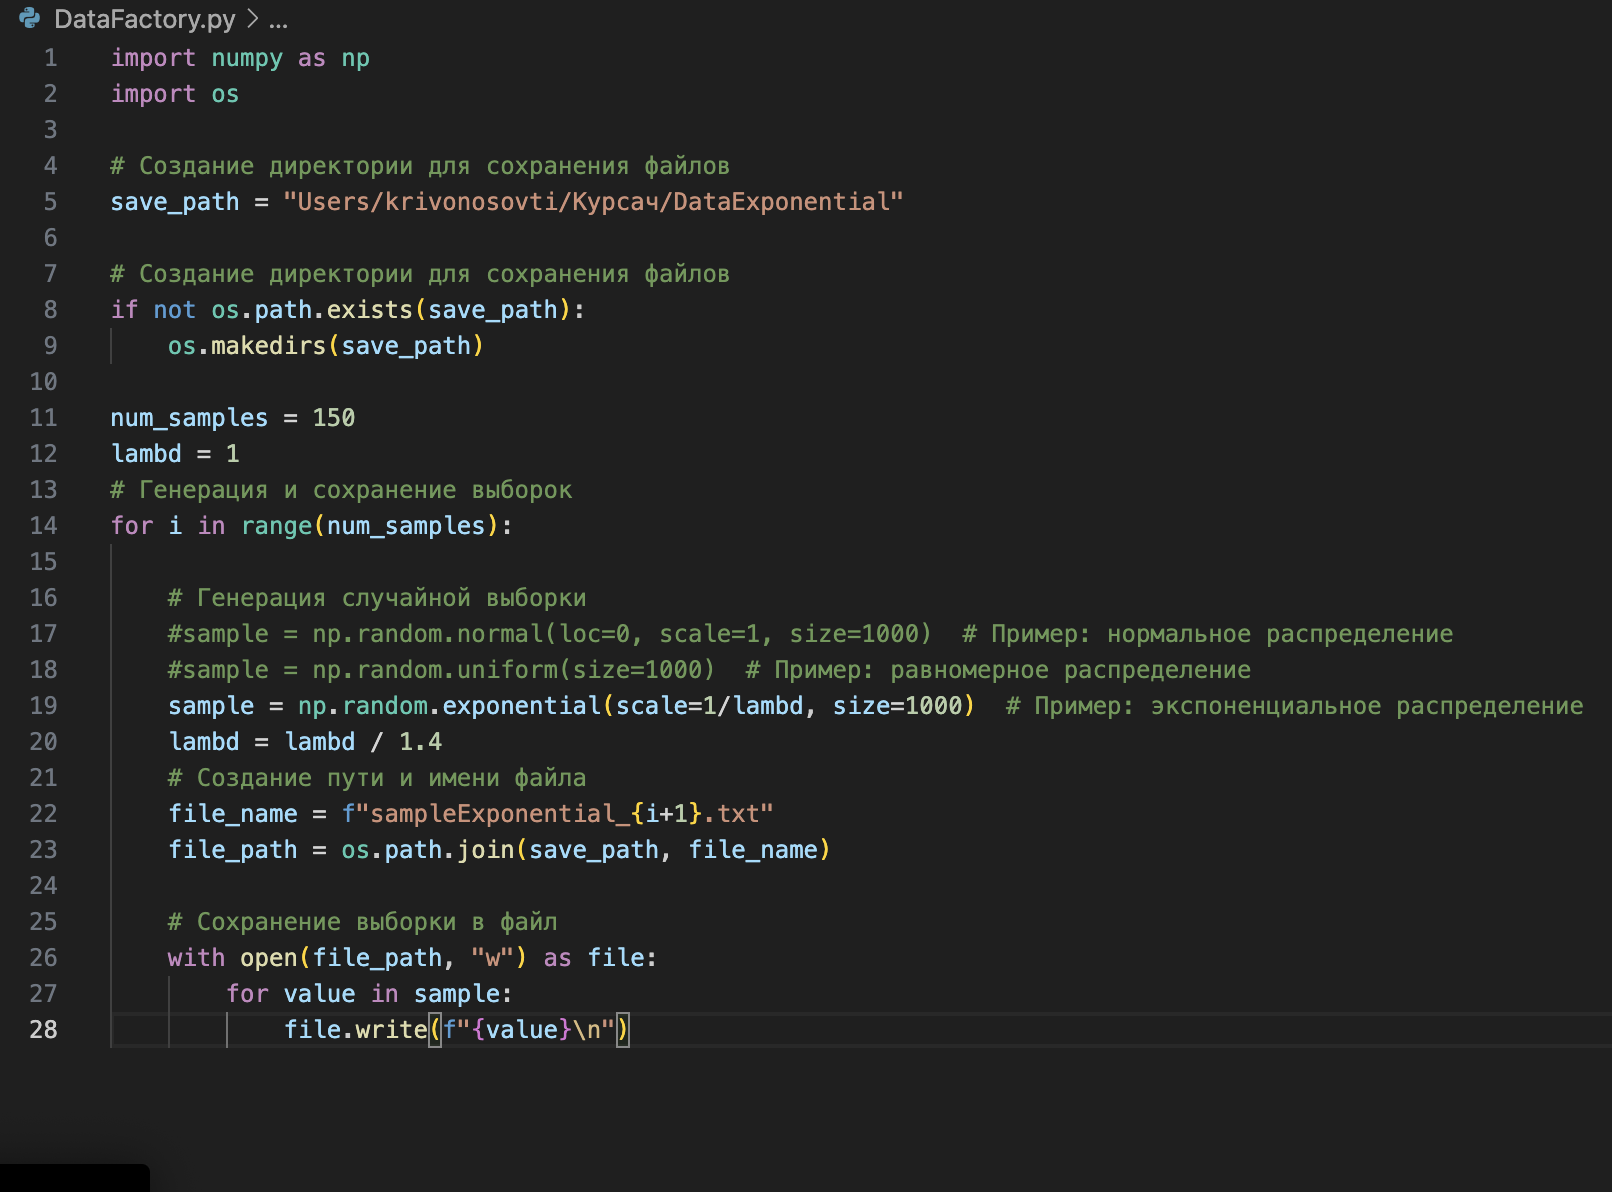
\includegraphics[width = 6in]{image1.png}
    \item Дельта метод углубленно
        \label{sec: Приложение 2}
        Методолгия:
        Предположим, что A/B-тест задается с несколькими вариантами, где кандидаты в каждом варианте получают разный опыт. Мы заинтересованы в измерении того, как
        
        Опыт в каждом варианте влияет на q-й квантиль времени загрузки страницы. Чтобы измерить это влияние и вычислить статистическую значимость, нам нужны оценки количества выборки и стандартного отклонения квантиля выборки в каждом варианте. При увеличении одного варианта, предположим, что в этом варианте есть:
        
        Участники $i = 1,2,3,  ... , n$

        Страници просмотренные i-ым участником $j = 1, 2, 3, ... ,\textit{P}{i}$, где $\textit{P}{i}$ (i.i.d) случайные значения удовлетворяющие функции распрелеления $\mathcal{P}$.

        Загрузка j-ой страницы i-ым участником = $\textit{X}{ij}$   

        q-ый выборочный квантиль $\{\textit{X}{ij}, i = 1,2,...n; j = 1,2,3, ... ,  \textit{P}{i} \}$ обозначим как $\widehat{Q}$ 

        Дисперсия - $Var(\widehat{Q} )$; стандартное откланение $stddev(\widehat{Q})$


        
\includegraphics[width = 6in]{IMG_0086.jpg}
        \newline
        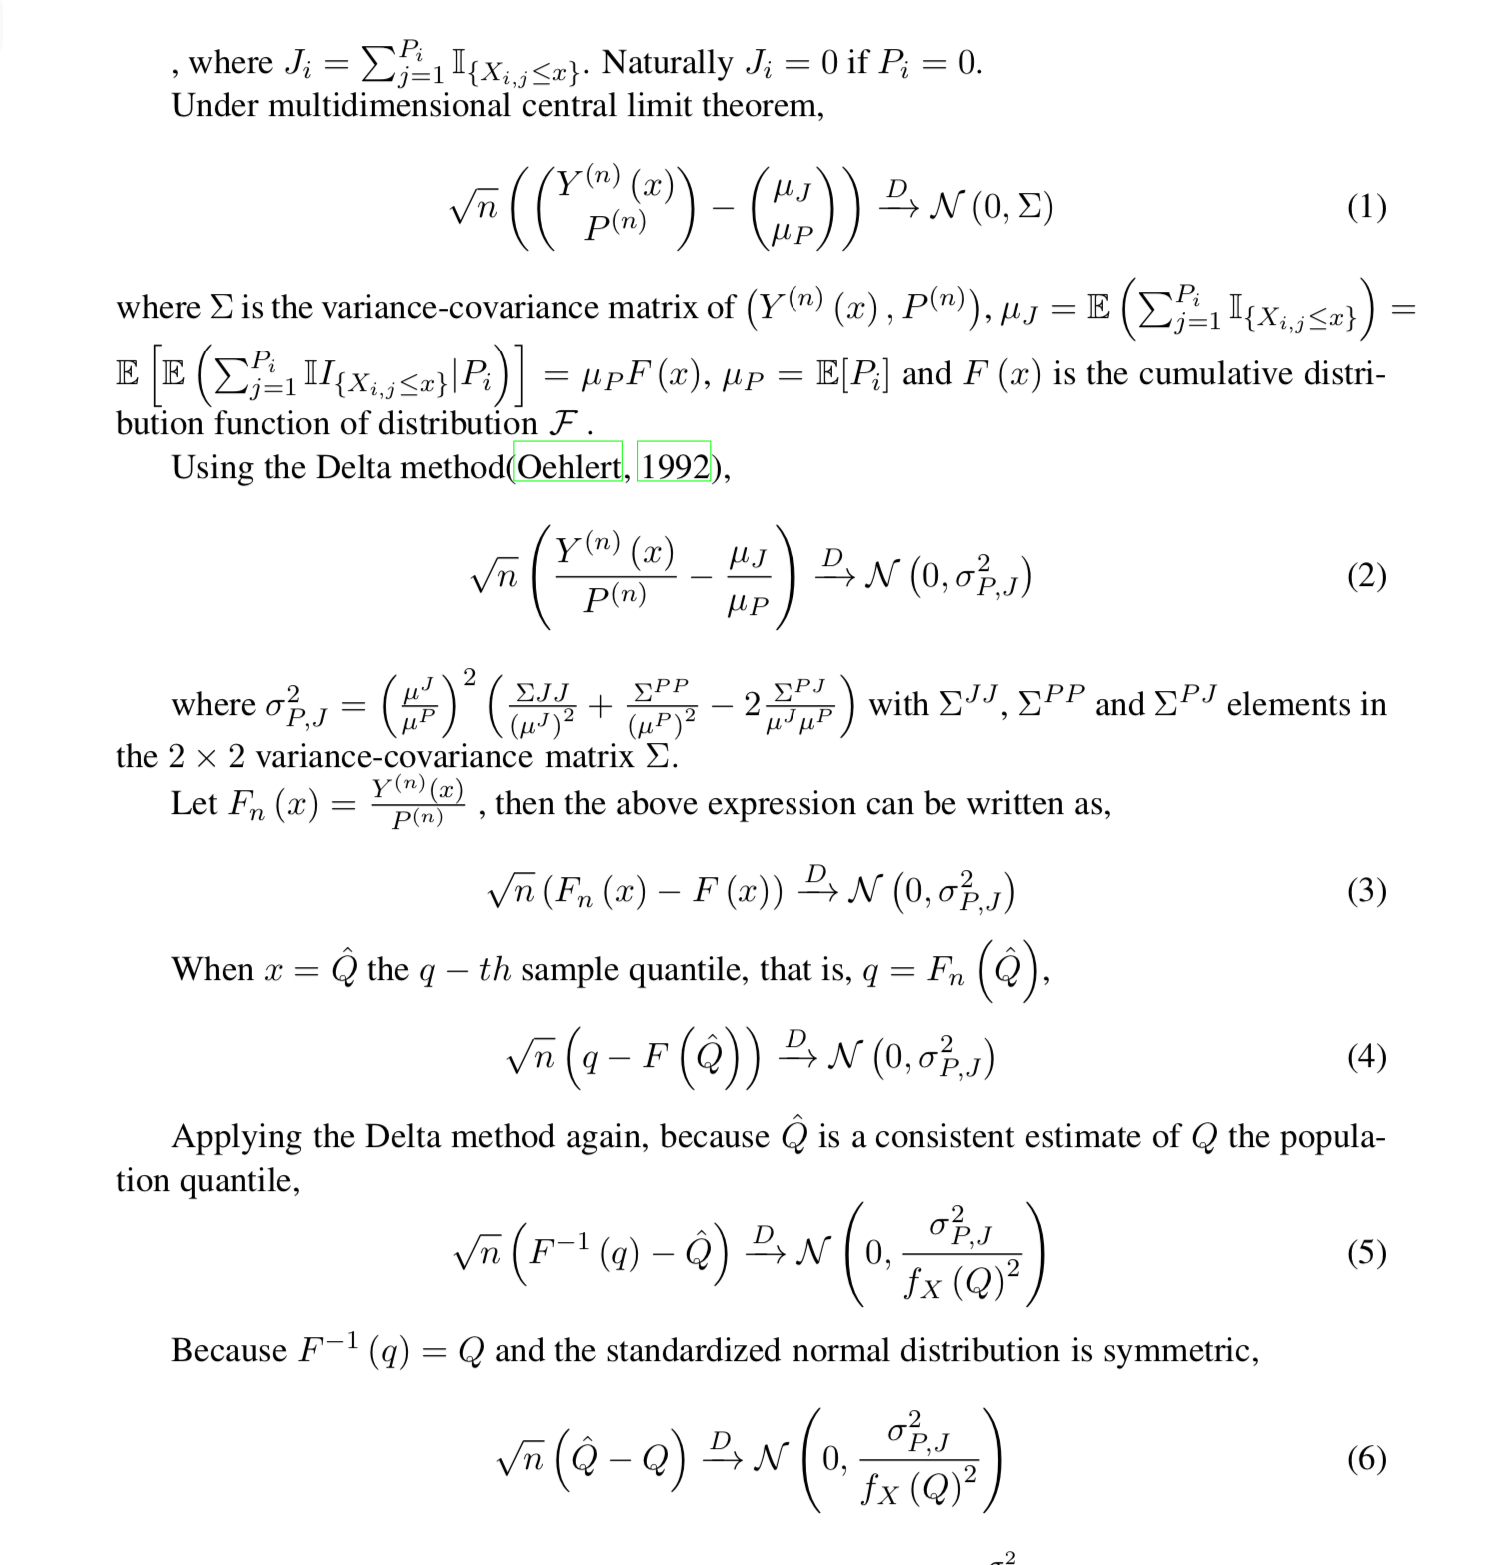
\includegraphics[width = 6in]{IMG_D1552B1059C6-1.jpeg}
        
        // тут должна быть антотация вставки 

        Таким образом асимптотическая оценка дисперисии кванитиля это $\frac{\sigma ^ 2_{P,J}}{nf_{X}(Q)^2}$,  где Q можно оценить со средней плотностью в небольшом доверительном интевале $\widehat{Q}$.

        Предположим, что из n участников только  $i = 1, 2,...,n_0$  имет ненулевые просмотры на интересующей странице.
        
        Определим: 
        
        $\mu_0^J = E(J_i|i =1,2, ... , n_0)$; $\mu_0^P = E(P_i|i =1,2, ... , n_0)$; $\Sigma_0 = Cov(J_i,P_i|i = 1,2,...,n_0)$
        Тогда:

        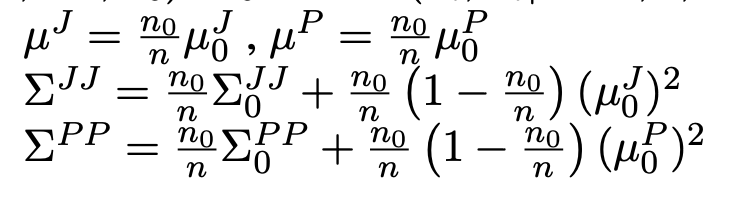
\includegraphics[width = 3in]{Снимок экрана 2023-10-16 в 22.09.59.png}

        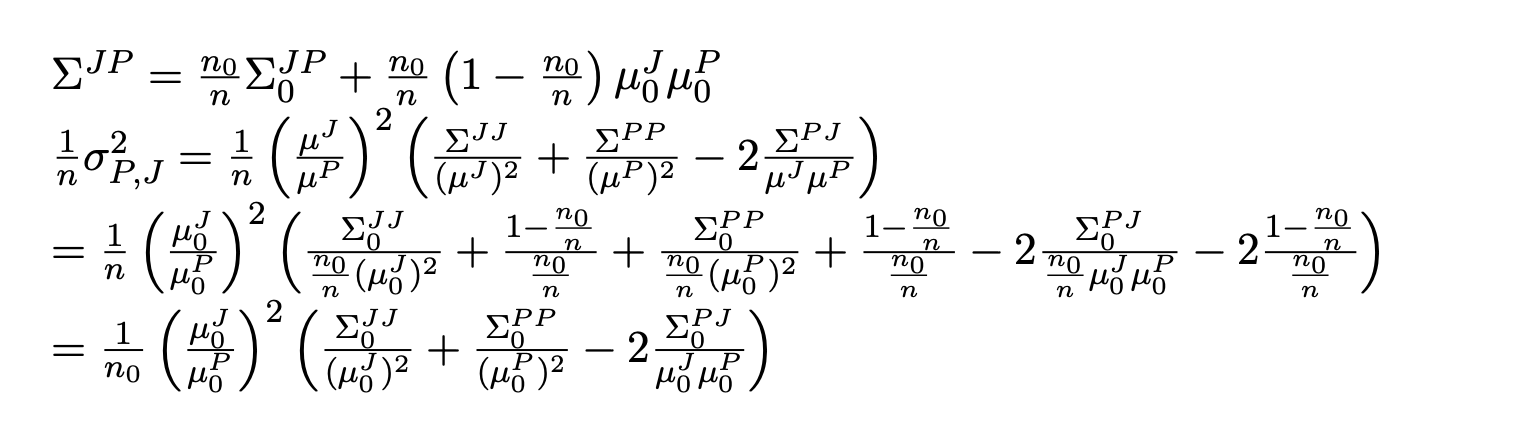
\includegraphics[width = 6in]{Снимок экрана 2023-10-16 в 22.10.53.png}
        \newline
    
    
    \end{enumerate} 
        
\end{document}